\documentclass[byrevtex,amssymb,aps,pra,floatfix,letterpaper]{revtex4}
\usepackage{graphicx}
\usepackage{hyperref}
\usepackage{verbatim}
\bibliographystyle{apsrev}
\date{\today}
\pagestyle{plain}
\newcommand{\degree}[0]{$^\circ$}

\begin{document}

\title{Experiment 3: Cyclic Voltammetry}

\date{\today}

\maketitle

\section{Introduction}

Redox reactions of quinone compounds have found application in many areas of chemistry and biology, such as photosynthesis \cite{BIOCHEM1}, anthracycline cytostatic drugs \cite{BIOCHEM2}, and wood and paper chemistry \cite{PAPER1}. In this exercise cyclic voltammetry is used to study the redox processes and solvent hydrogen bonding effects in 2,3,5,6-tetramethyl-1,4-benzoquinone (duroquinone; see Fig. \ref{fig1}) \cite{LINSCHITZ,WIGAL,GONZALEZ}. The importance of hydrogen bonding in physico-chemical processes is enormous. For example, the liquid state of water and the helical structure of DNA are attributed to hydrogen bonding.

\begin{figure}[!htp]
\begin{center}
\includegraphics[scale=0.5]{quinone}
\caption{Stucture and reduction scheme of duroquinone. The structure shown for the anion radical is one of the two possible resonance structures, where the unpaired electron and the negative charge may exchange. Note that the neutral species is not aromatic.}
\label{fig1}
\end{center}
\end{figure}

Voltammetry is a collection of electro-analytical techniques in which information about the analyte or a physical processe is derived from the measurement of current as a function of applied potential. It is widely used by chemists for non-analytical purposes including fundamental studies on redox processes, adsorption processes on surfaces, electron transfer mechanisms, and electrode kinetics.

\section{Cyclic voltammetry}

Voltammetric measurements are carried out using an electrochemical cell made up of three electrodes immersed in a solution containing the analyte and an excess of a nonreactive electrolyte called the supporting electrolyte. One of the three electrodes is the working electrode, which is typically made of platinum, gold, silver, glassy carbon, nickel, or palladium. The redox process occurs at this electrode. Its dimensions are kept small in order to enhance its tendency to become polarized. The second electrode is the reference electrode, which provides calibration for the applied potential. Examples of commonly used references are the normal hydrogen electrode, Ag/AgCl electrode, and calomel electrode (i.e., Hg/Hg$_2$Cl$_2$). The third electrode is the counter electrode, which is often a platinum wire that simply serves to conduct electricity from the signal source through the solution to the other electrodes. An example of a voltammetric setup is
shown in Fig. \ref{fig2}. Note that in absence of any redox processes, the electrodes behave like capacitor plates, which polarize the ions in the solution. This results in a small, but measurable, capacitive current in the system.

\begin{figure}[!htp]
\begin{center}
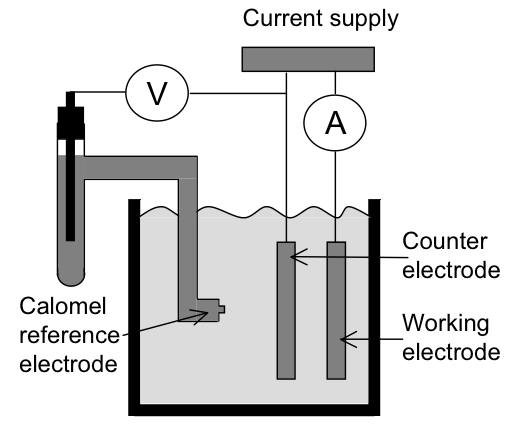
\includegraphics[scale=0.3]{cell}
\caption{An electrochemical cell. 'V' denotes a high impedance voltmeter (no current flows between the reference and working electrodes) and 'A' measures the current between the working and the counter electrodes. In a cyclic voltammetry experiment, the potential of the reference electrode is varied and the current between the working and reference electrodes is measured.}
\label{fig2}
\end{center}
\end{figure}

\begin{figure}[!htp]
\begin{center}
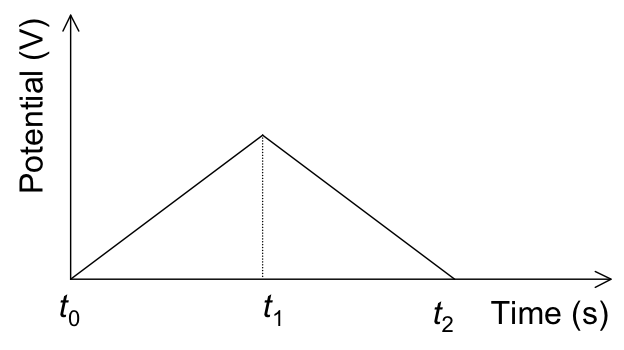
\includegraphics[scale=0.3]{triangle}
\caption{A triangular waveform is applied to the working electrode. For description of the symbols, see text.}
\label{fig3}
\end{center}
\end{figure}

\begin{figure}[!htp]
\begin{center}
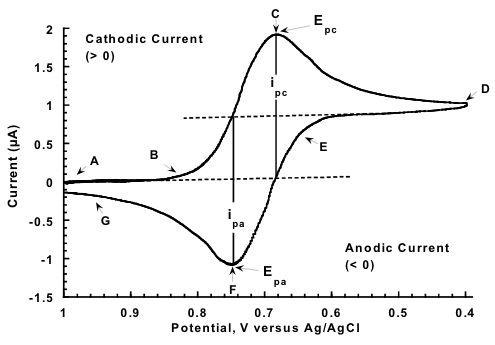
\includegraphics[scale=0.4]{voltammogram}
\caption{A typical cyclic voltammogram. For explanation of the symbols, see text.}
\label{fig4}
\end{center}
\end{figure}

Fig. \ref{fig3} shows the nature of the triangular voltage waveform that is applied to the working electrode. After applying a linear voltage ramp between $t_0$ and $t_1$, the ramp is reversed to bring the potential back to its initial value at time $t_2$. Fig. \ref{fig4} illustrates a typical cyclic voltammogram. In the parts of the wave labeled 'A', 'B', and 'C', the potential is applied and an increasing amount of current is observed. This is the cathodic part of the
wave, where reduction of the quinone molecules is occurring. Maximum flow of electrons is observed at point 'C'. After point 'C', potential is still applied, but the current associated with the reduction decreases due to a depletion of quinone molecules at the electrode. Quinone diffusion toward the electrode must occur before reduction. Here diffusion is slower than reduction and therefore there is a reduction in the current flow between the parts 'C' and 'D'. Parts 'E', 'F', and 'G' describe the reverse process (i.e., the anodic part). When the voltage is decreased, the reverse oxidation process occurs, and the quinone molecules are returned to their initial state. Fig. \ref{fig5} demonstrates a typical cyclic voltammogram for a two-electron reduction process, where one peak is observed
on both sides for each electron transfer process.

\begin{figure}[!htp]
\begin{center}
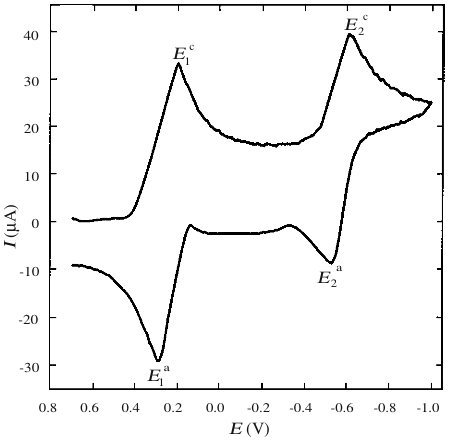
\includegraphics[scale=0.4]{voltammogram2}
\caption{A two-electron voltammogram. $E_1^c$ and $E_2^c$ denote the current maxima on the cathodic wave and $E_1^a$ and $E_2^a$ for the anodic wave.}
\label{fig5}
\end{center}
\end{figure}

The redox potential can be obtained from a voltammogram by calculating the average value of the anodic and cathodic peaks. For example, for the voltammogram
shown in Fig. \ref{fig5}, the one-electron ($E_{1,1/2}$) and two-electron ($E_{2,1/2}$) redox potentials can be calculated as:

\begin{equation}
\label{eq1}
E_{1,1/2} = \frac{E_1^c + E_1^a}{2}\textnormal{ and }E_{2,1/2} = \frac{E_2^c + E_2^a}{2}
\end{equation}

\noindent
The subscript $1/2$ indicates that the potential is obtained approximately at the half-height of the cathodic and anodic peaks and hence is sometimes called the half-wave potential. At these points the concentrations of the reduced and oxidized species are equal. Note that in this context concentration refers to concentration of a given species on the electrode -- not in the bulk solution. In cases where only one-electron reduction occurs, only one maximum is observed in the cathodic and one minimum in the anodic waves. When the anodic and cathodic waves are symmetric with respect to each other, the redox process is reversible. If they are not symmetric, the redox species may undergo a chemical reaction and will not be observed on the returning sweep. Remember that the measured values are
always expressed relative to the reference electrode and appropriate conversions must be carried out when comparing with data taken with a different type of reference electrode.

\section{Determination of the redox potential and the degree of hydrogen bonding in duroquinone}

The purpose of this experiment is to determine the redox potential of duroquinone (i.e., the potential governing the formation of anion radicals and dianions as shown in Fig. \ref{fig1}) and to determine the number of CH$_3$CH$_2$OH (ethanol) molecules hydrogen bonding to the quinone oxygens at positions 1 and 4. The largest partial charges reside on the quinone oxygens and on the alcoholic proton of ethanol. This promotes the formation of hydrogen bond between them. Recall that hydrogen bonding arises from the electrostatic interaction between opposite partial charges in molecules. The strength of hydrogen bonding depends on the magnitudes of the attracting partial charges as well as possible steric effects for molecular approach.

Benzoquinone and its substituted derivatives (denoted by $Q$) undergo reversible two step-wise one-electron transfer reactions in aprotic (i.e., non-proton donating) solvents. Examples of aprotic solvents are acetonitrile (CH$_3$CN), benzonitrile, dimethylsulfoxide (DMSO), dimethylformamide (DMF). The reduction scheme is shown in Fig. \ref{fig1}. In the presence of a protic (i.e., proton donating; denoted by $S$) solvent, association of solvent molecules to $Q$ must be considered \cite{GONZALEZ}:

\begin{eqnarray}
\label{eq2}
& & \textnormal{For the anion radical:}\\
\nonumber
& & Q^{\cdot-} + S \rightleftharpoons Q^{\cdot-}\cdot\cdot\cdot S\\
\nonumber
& & Q^{\cdot-} + 2S \rightleftharpoons Q^{\cdot-}\cdot\cdot\cdot S_2\\
\nonumber
& & \textnormal{. . .}\\
\nonumber
& & Q^{\cdot-} + nS \rightleftharpoons Q^{\cdot-}\cdot\cdot\cdot S_n\\
\nonumber
& & \textnormal{and for the dianion:}\\
\nonumber
& & Q^{2-} + S \rightleftharpoons Q^{2-}\cdot\cdot\cdot S\\
\nonumber
& & Q^{2-} + 2S \rightleftharpoons Q^{2-}\cdot\cdot\cdot S_2\\
\nonumber
& & \textnormal{. . .}\\
\nonumber
& & Q^{2-} + mS \rightleftharpoons Q^{2-}\cdot\cdot\cdot S_m
\end{eqnarray}

\noindent
where the association of solvent molecules up to $n$ and $m$ is shown. In this work, we assume that only one hydrogen bonded form dominates for $Q^{\cdot−}$ and $Q^{2-}$ \cite{LINSCHITZ}:

\begin{eqnarray}
\label{eq3}
& & Q^{\cdot-} + nS \rightleftharpoons Q^{\cdot-}\cdot\cdot\cdot S_n\\
\nonumber
& & Q^{2-} + mS \rightleftharpoons Q^{2-}\cdot\cdot\cdot S_m
\end{eqnarray}

\noindent
where symbol $n$ denotes an average number of protic solvent molecules bound to the anion radical and $m$ is the corresponding number for the dianion. Note that both (\ref{eq2}) and (\ref{eq3}) are simplified schemes in a sense that the actual redox processes occur for solvated forms of $Q$ and $Q^{\cdot-}$ (i.e., for $Q\cdot\cdot\cdot S_i$ and $Q^{\cdot-}\cdot\cdot\cdot S_j$) and therefore the redox potentials also shift to lower energy (i.e., the redox process occurs more easily). The equilibrium constants for (\ref{eq3}) can be written as:

\begin{equation}
K_1 = \frac{\left[Q^{\cdot-}\cdot\cdot\cdot S_n\right]}{\left[Q^{\cdot-}\right]\left[S\right]^n}\textnormal{ and }
K_2 = \frac{\left[Q^{2-}\cdot\cdot\cdot S_m\right]}{\left[Q^{2-}\right]\left[S\right]^m}
\label{eq4}
\end{equation}

\noindent
Note that the assumption of single solvation form may introduce values for $n$ and $m$ that are not integers and thus they should be interpreted as average values for the associated solvent molecules. The effect of solvent molecules on the redox potential can be derived as follows:

\noindent
1. \textit{The anion radical} (i.e., the first line in (\ref{eq3})). The total concentration of anion radical is given by:

\begin{equation}
\left[Q^{\cdot-}\right]_{total} = \left[Q^{\cdot-}\right] + \left[Q^{\cdot-}\cdot\cdot\cdot S_n\right]
\label{eq5}
\end{equation}

\noindent
By expressing this in terms of the equilbrium constant $K_1$ (see (\ref{eq4})), we get:

\begin{equation}
\left[Q^{\cdot-}\right]_{total} = \left[Q^{\cdot-}\right]\times\left(1 + K_1\left[S\right]^n\right)
\label{eq6}
\end{equation}

\noindent
Assuming that the electrochemical reactions are reversible, the Nernst equation for the redox pair $Q/Q^{\cdot-}$ can be written:

\begin{equation}
E_1 = E_1^\circ + \frac{RT}{NF}\ln\left(\frac{\left[Q\right]}{\left[Q^{\cdot-}\right]}\right)
\label{eq7}
\end{equation}

\noindent
where $E_1$ is the effective redox potential when protic solvent $S$ is present (V), $E_1^\circ$ is the standard redox potential in aprotic solvent (i.e., without S; units in V), $R$ is the molar gas constant (8.31451 J mol$^{-1}$ K$^{-1}$), $T$ is the cell temperature (K), $N$ is the number of electrons transferred (i.e., here $N$ = 1) and $F$ is the Faraday constant (9.648531 $\times$ $10^4$ C mol$^{-1}$). Note that only the non-hydrogen bonded form is involved in the reduction process as the hydrogen bonding occurs after the reduction. Inserting Eq. (\ref{eq6}) in Eq. (\ref{eq7}), we get:

\begin{eqnarray}
& & E_1 = E_1^\circ + \frac{RT}{NF}\ln\left(\frac{\left[Q\right]}{\left[Q^{\cdot-}_{total}\right]}\times\left(1 + K_1\left[S\right]^n\right)\right)\\
\nonumber
& & = E_1^\circ + \frac{RT}{NF}\ln\left(\frac{\left[Q\right]}{\left[Q^{\cdot-}\right]_{total}}\right) + \frac{RT}{nF}\ln\left(1 + K_1\left[S\right]^n\right)
\label{eq8}
\end{eqnarray}

\noindent
At the half-wave potential the total concentrations of the oxidant and the reductant are equal (i.e., $\left[Q\right] = \left[Q^{\cdot-}\right]$) and $E_1$ becomes $E_{1,1/2}$. Thus Eq. (\ref{eq8}) now becomes (with $N = 1$):

\begin{equation}
E_{1,1/2} = E_{1,1/2}^o + \frac{RT}{F}\ln\left(1 + K_1\left[S\right]^n\right)
\label{eq9}
\end{equation}

\noindent
When the hydrogen bonded form dominates (i.e., $K_1 \times \left[S\right]^n >> 1$; see Eq. (\ref{eq4})) and the half-wave potential shift is denoted by $\Delta E_{1,1/2} = E_{1,1/2} - E_{1,1/2}^\circ$, the above equation can be simplified as:

\begin{eqnarray}
& & E_1{1,1/2} = E_{1,1/2}^\circ + \frac{RT}{F}\ln\left(K_1\left[S\right]^n\right) = E_{1,1/2}^\circ + \frac{RT}{F}\ln\left(K_1\right) + \frac{nRT}{F}\ln\left(\left[S\right]\right)\\
\nonumber
& & \Rightarrow \Delta E_{1,1/2} = E_{1,1/2} - E_{1,1/2}^\circ = \underbrace{\frac{RT}{F}\ln\left(K_1\right)}_{\textnormal{``b''}} + \underbrace{\frac{nRT}{F}\ln\left(\left[S\right]\right)}_{\textnormal{``kln(x)``}}
\label{eq10}
\end{eqnarray}

\noindent
Thus plotting logarithm of the concentration $\left[S\right]$ on the $x$-axis and $\Delta E_{1,1/2}$ on the $y$-axis should yield a straight line (''$y = b + k\ln(x)$``). Fitting the experimental $\Delta E_{1,1/2}$ points obtained with various concentrations $\left[S\right]$ yields estimates for both the equilibrium
constant $K_1$ and the average number of hydrogen bonded solvent molecules $n$. The experimental half-wave potentials must be extracted from the voltammograms using Eq. (\ref{eq1}).\\

\noindent
2. \textit{The dianion} (see 2nd line in Eq. (\ref{eq3})).\\

\noindent
This case proceeds in a similar way as case 1 above. First, we write the total concentration for the dianion:

\begin{equation}
\left[Q^{2-}\right]_{total} = \left[Q^{2-}\right] \times \left(1 + K_2\left[S\right]^m\right)
\label{eq11}
\end{equation}

\noindent
By writing the Nernst equation for the $Q^{\cdot-}/Q^{2-}$ redox pair and carrying out similar algebra that we did in deriving Eq. (\ref{eq9}), we get ($N = 1$):

\begin{eqnarray}
& & E_{2,1/2} = E_{2,1/2}^\circ + \frac{RT}{F}\ln\left(\frac{\left[Q^{\cdot-}\right]}{\left[Q^{2-}\right]}\right)
 = E_{2,1/2}^\circ + \frac{RT}{F}\ln\left(\frac{1 + K_2\left[S\right]^m}{1 + K_1\left[S\right]^n}\right)
 \approx E_{2,1/2}^\circ + \frac{RT}{F}\ln\left(\frac{K_2}{K_1}\left[S\right]^{m-n}\right)\\
\nonumber
& & \Rightarrow \underbrace{\Delta E_{2,1/2}}_{\textnormal{''y``}} = E_{2,1/2} - E_{2,1/2}^\circ = \underbrace{\frac{RT}{F}\ln\left(\frac{K_2}{K_1}\right)}_{\textnormal{''b``}} + \underbrace{\frac{RT(m - n)}{F}\ln\left(\left[S\right]\right)}_{\textnormal{''kln(x)``}}
\label{eq12}
\end{eqnarray}

\noindent
This is again a straight line when plotted against logarithm of the concentration $\left[S\right]$. Fitting would yield estimates for the ratio of $K_2 / K_1$ and the difference $m - n$. Values for $K_1$ and $n$ are known from the anion radical data (previous case) and therefore values for $m$ and $K_2$ can be calculated using Eq. (\ref{eq12}).

\section{Experimental}

\noindent
\underline{Instrument:} A EG\&G Potentiostat / Galvanostat controlled by a computer through Power Suite software (''echem program``). The sofware has a provision for carrying out Cyclic Voltammatry, storing, overlaying and printing graphs.\\

\noindent
\underline{Electrodes:} Working electrode: glassy carbon (Bioanalytical systems, 6 mm diameter); Counter electrode: Pt electrode; Reference electrode: Ag wire (''quasi electrode``). For the latter, a standard Ag/AgCl, SCE or Ag/AgNO$_3$ electrode can also be used.\\

\noindent
\underline{Chemicals:} Quinone (duroquinone; M.W. 164.21 g mol$^{-1}$), Tetra-$n$-butylammonium hexafluorophosphate (TBAHFP; M.W. 387.44 g mol$^{-1}$), acetonitrile (aprotic solvent; dried over drierite), dry ethanol (Fisher reagent grade dried over molecular sieves; protic solvent; denoted by $S$ previously).\\

\noindent
\underline{Task overview:} You will record cyclic voltammograms (CVs) of a 2 mM solution of quinone in dry acetonitrile (25 mL; do not shake!). You will add successive amounts of dry ethanol to the solution in the cell to make 0.05 M, 0.1 M, 0.2 M, 0.5 M and 1.0 M in ethanol. In order to get the correct ethanol concentrations, you will need to use the molecular weight of ethanol (46.0634 g mol$^{-1}$) and density of ethanol (0.789 g mL$^{-1}$). The initial amount of solution in the CV cell will be 10 mL. Be sure to make the required calculations in advance (i.e., how much ethanol will need to be added at each step). The
amount for the first addition is some tens of $\mu$L. Finally, the solution in the CV cell will have to be purged to remove oxygen by bubbling nitrogen gas after each successive addition of EtOH.\\

\noindent
\underline{Laboratory cautions for cyclic voltammetry:}\\

\noindent
\begin{enumerate}
\item Contamination of reagents, glassware or electrodes can be a serious problem in this experiment. Make sure that only the pure reagents identified for this experiment are used and that all glassware and electrode surfaces are thoroughly clean before proceeding.

\item When you are finished using the electrode assembly, thoroughly rinse the cell and electrodes, clean the working electrode by rubbing it very gently with a very fine emery paper, washing it with deionized water and then with acetonitrile or ethanol. Clean the jacket of the reference electrode by throwing out the contents of the jacket and rinsing with acetonitrile. Also wash the silver wire and counter electrode with acetonitrile.

\item The last person using the nitrogen gas for purging must close the valve to the tank before leaving.

\end{enumerate}

\underline{The experimental procedure:}\\

\begin{enumerate}

\item Prepare 25.0 mL of a 2.0 mM solution of quinone ($<$ 10 mg needed) with 0.1 M TBAHFP ($<$ 1 g needed) as the supporting electrolyte in acetonitrile using a 25 mL volumetric flask. Do not wash anything with water. Make sure the solution is mixed well and that all solids have been dissolved.

\item Prepare the sample and install the electrodes:
\begin{enumerate}
\item Assemble the reference electrode (''R``). Insert the jacket of reference electrode in one of the holes of the stopper. If the silver wire is not shiny use a fine emery paper to clean the surface and then wipe it with ‘kimwipe'.
\item Take a look at the working electrode surface (''W``). If the surface is not mirror shiny, notify the instructor. In this case the electrode needs polishing: put a drop of distilled water on a 1500 grade emery paper and gently rub the electrode surface on the emery paper rotating it in clock and then counter-clock directions 5 - 6 times. Wash the surface of the electrode and dry with kimwipe. The electrode should be as shiny as a mirror. If not, the electrode needs more polishing.
\item Deliver 10.0 mL of the 2.0 mM solution to the voltammetric cell.
\item Insert the counter (''C``) and working electrodes in the two holes of the stopper and stopper the cell. Insert the reference electrode in the jacket of the reference electrode.
\item Bubble the solution with N$_2$ for 5 - 10 min.
\end{enumerate}

\item Start the CV program by double clicking on ''EpsilonEC-20...``. Set the instrument mode to CV by selecting Experiment$\rightarrow$Select New Experiment and select Cyclic Voltammetry (CV) mode from the list and click Select. Set the parameters as follows: Initial Potential (mV): 200, Switching Potential (mV): -2200, Final Potential (mV):
200, \# of Segments: 2, Scan Rate (mV/s): 100, Quiet Time (s): 2, Full Scale (+/-): 100 $\mu$A; finally click on Apply. Purge the sample by choosing Experiment$\rightarrow$Manual Settings. In the appearing dialog set Purge (s): 600 and click Apply right next to the purge settings. The timer will go to zero when the sample is ready for measurement. Click Exit after purging is done. To run the measurement, click on Run at the top bar in the main window. After the measurement is done, click on the Print button at the top part of the main window. The program will automatically indicate the important readings on the graph.These values are required to use Eq. (\ref{eq1}). Remember also to write down what sample the file corresponds to, concentrations, etc.

\item Using a microsyringe, add the proper amount of dry ethanol to the solution in the cell to make it 0.05 M in ethanol and bubble the solution for 5 - 10 min with N$_2$ gas. Measure the sample, record the peak maxima, and save and print a copy of the voltammogram. This should be done as instructed above.

\item Using the microsyringe, deliver the proper amount of ethanol to the same solution in the cell to increase the total ethanol concentrations to 0.1 M, 0.2 M, 0.5 M and 1.0 M. Make sure to deoxygenate the solution with nitrogen every time. Make sure to save each voltammogram and record the required values from the voltammogram.

\end{enumerate}

\section{Data analysis}

Calculate the $E_{1,1/2}$ and $E_{2,1/2}$ values using Eq. (\ref{eq1}) for each sample (i.e., each ethanol concentration) and present the data ($\Delta E_{1,1/2}$ vs. $\left[S\right]$ and $\Delta E_{2,1/2}$ vs. $\left[S\right]$) in tabular form. Use the qtiplot program to fit your data:

\begin{enumerate}
\item Start qtiplot

\item  Enter your data into the empty table1. Enter first $\Delta E_1$ for the five samples. The X column is concentration and Y column is $\Delta E_1$. Then in the same table immediately after $\Delta E_1$ data, continue to enter the $\Delta E_2$ data the same way. For example, your table should look like:

\begin{verbatim}
   X     Y
   0.05	 0.031
   0.1	 0.037
   0.2	 0.073
   0.5	 0.088
   1.0	 0.110
   -0.05 0.167
   -0.1	 0.172
   -0.2	 0.296
   -0.5	 0.378
   -1.0	 0.462
\end{verbatim}

Note that all the delta values should be positive.

\item  Perform non-linear fit of the data. Select the Y column in table1. Choose ''Analysis $\rightarrow$ Fit Wizard``. If you get ''Choose the plugins folder`` dialog, just click the Open button to close it. Type into the large box at the bottom of the appearing dialog:

\begin{verbatim}
 if(x<0,
   (8.31451*298/96485.31)*log(1.0+K1*(abs(x)^n)),
   (8.31451*298/96485.31)*log((1.0+K2*(abs(x)^m))/(1.0+K1*(abs(x)^n)))
   )
\end{verbatim}

Be careful when typing it as mismatched parentheses etc. will cause errors. Note that we are fitting two datasets with shared parameters. The first set is at positve X values and the second set at negative X values. The abs() functions were put in place to make sure that the X values will be positive. Confirm that the above formulas are the same as given in the lab manual. Hit ''Fit $>>$`` to continue to the fitting menu. Give the following initial values for the parameters:   $K_1 = 1e+5, K_2 = 1e+12, m = 5, n = 5$.  Click on ''Fit`` button. Graph1 will show the experimental data points along with the fitted function. The results.log window at the top will contain the values of the parameters (i.e., $K_1,K_2,m,n$), their error estimates, and the $r^2$ value. Write down these values. Note that you can scroll this window up. If your calculation does not converge, try changing the above initial guess.

\item You can modify the graph to have the correct X/Y axes, title, etc. by double clicking on these areas on the graph. To modify the curve settings, double click on the curves. You may want to display just data points rather than the continuous lines. The graph legend can be modified by double clicking on it. In the legend \textbackslash l(1) corresponds to the line style of the first curve and \textbackslash l(2) to the second curve.

\item To print out the graph, select the window and choose ''File $\rightarrow$ Print``.

\end{enumerate}

The above procedure has fitted Eqs. (\ref{eq9}) and (\ref{eq12}) to your experimental data. Note that this did not make the following assumptions: $K_1 \times \left[S\right]^n >> 1$ and $K_2 \times \left[S\right]^m >> 1$. The program uses a non-linear least squares routine and the function may therefore have any form. The limiting forms (Eqs. (\ref{eq10}) and the last part of (\ref{eq12})) were given just to illustrate the behavior of the data sets. You would use them when you don't have access to a computer with data analysis software, you are using a linear least squares routine or the resulting non-linear fitting experiences
convergence problems. 

\section{Written laboratory report}

Follow the general instructions for written laboratory reports. In addition, include the requested data in the following section:\\

\noindent
\textit{Results.} This section should include the values for $m$, $n$, $K_1$ and $K_2$ and their error estimates. Include the graphs obtained from the non-linear least squares analysis. Find the literature values for these quantities \cite{LINSCHITZ} (note: different solvent!) and discuss the possible sources of errors. Provide a schematic drawing how the protic molecules might be hydrogen bonded to the quinone molecule.\\

\noindent
\textit{Acknowledgment:} The CSUN Chemistry Department wishes to thank Dr. M. Mohammad and S. Toner for their contribution to this experiment.

\section{References}

\vspace{-1cm}

\bibliography{../references}

\end{document}
